\begin{problem}{1}
	Szachownicę o wymiarach $15 \times 15$ przykryto przy pomocy płytek o wymiarach $2 \times 2$ i $3 \times 3$ w taki sposób, że każde pole jest przykryte przez dokładnie jedną płytką oraz płytki nie wystają poza szachownicę. Wyznaczyć najmniejszą liczbę użytych płytek $3 \times 3$, dla której jest to możliwe.
\end{problem}

\begin{problem}{2}
	Płaszczyznę pokolorowano trzema kolorami. Wykazać, że istnieje odcinek o długości $1$, który ma końce tego samego koloru.
\end{problem}

\begin{problem}{3}
	Czy można wypełnić szachownicę o wymiarach $8 \times 8$ przy pomocy jednego $Z$-klocka oraz dowolnej liczby prostokątów $1 \times 4$.
	\begin{center}
	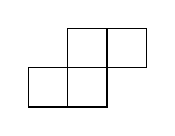
\begin{tikzpicture}[scale=0.5]
		\draw (0,0) -- (2,0) -- (2,1) -- (3,1) -- (3,2) -- (2,2) -- (2,1) -- (0,1) -- cycle;
		\draw (1,0) -- (1,2) -- (2,2);
	\end{tikzpicture}
\end{center}
\end{problem}

\begin{problem}{4}
	Sad podzielony jest na $100$ przystających kwadratów, tworzących szachownicę $10 \times 10$. Na dzięwieciu kwadratach znajduje się roślina. Co roku roślina rozrasta się na pola, które już sąsiadują -- mają wspólny bok -- z co najmniej dwoma polami, na których już rośnie roślina. Udowodnić, że roślina nigdy nie rozrośnie się tak, aby zajmować cały sad.
\end{problem}
 
\begin{problem}{5}
	Każdy punkt płaszczyzny pokolorowano jednym z dwóch kolorów. Wykazać, że istnieje taki trójkąt o kątach $80\degree$, $80\degree$ i $20\degree$, że wszystkie jego wierzchołki są jednego koloru.
\end{problem}


\begin{problem}{6}
	Prostokąt $\mathcal{P}$ o wymiarach $1001 \times 1001$, podzielono na pewną liczbę prostokątów, z których każdy ma boki długości całkowitej (przykład na rysunku). Wykazać, że z tych prostokątów można wybrać taki jeden, że odległości jego czterech boków od odpowiadających mu boków $\mathcal{P}$ albo są wszystkie liczbami parzystymi, albo są wszystkie liczbami nieparzystymi.

	\begin{center}
	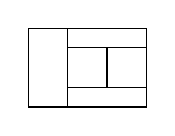
\begin{tikzpicture}[scale=0.5]
		\draw (0,0) -- (3,0) -- (3,2) -- (0,2) -- cycle;
		\draw (0,0) -- (1,0) -- (1,2) -- (0,2) -- cycle;
		\draw (1,0) -- (3,0) -- (3,0.5) -- (1,0.5) -- cycle;
		\draw (1,1.5) -- (3,1.5) -- (3,2) -- (1,2) -- cycle;
		\draw (2,0.5) -- (3,0.5) -- (3,1.5) -- (2,1.5) -- cycle;
	\end{tikzpicture}
\end{center}
\end{problem}


